\documentclass{article}\usepackage[]{graphicx}\usepackage[]{color}
%% maxwidth is the original width if it is less than linewidth
%% otherwise use linewidth (to make sure the graphics do not exceed the margin)
\makeatletter
\def\maxwidth{ %
  \ifdim\Gin@nat@width>\linewidth
    \linewidth
  \else
    \Gin@nat@width
  \fi
}
\makeatother

\definecolor{fgcolor}{rgb}{0.345, 0.345, 0.345}
\newcommand{\hlnum}[1]{\textcolor[rgb]{0.686,0.059,0.569}{#1}}%
\newcommand{\hlstr}[1]{\textcolor[rgb]{0.192,0.494,0.8}{#1}}%
\newcommand{\hlcom}[1]{\textcolor[rgb]{0.678,0.584,0.686}{\textit{#1}}}%
\newcommand{\hlopt}[1]{\textcolor[rgb]{0,0,0}{#1}}%
\newcommand{\hlstd}[1]{\textcolor[rgb]{0.345,0.345,0.345}{#1}}%
\newcommand{\hlkwa}[1]{\textcolor[rgb]{0.161,0.373,0.58}{\textbf{#1}}}%
\newcommand{\hlkwb}[1]{\textcolor[rgb]{0.69,0.353,0.396}{#1}}%
\newcommand{\hlkwc}[1]{\textcolor[rgb]{0.333,0.667,0.333}{#1}}%
\newcommand{\hlkwd}[1]{\textcolor[rgb]{0.737,0.353,0.396}{\textbf{#1}}}%
\let\hlipl\hlkwb

\usepackage{framed}
\makeatletter
\newenvironment{kframe}{%
 \def\at@end@of@kframe{}%
 \ifinner\ifhmode%
  \def\at@end@of@kframe{\end{minipage}}%
  \begin{minipage}{\columnwidth}%
 \fi\fi%
 \def\FrameCommand##1{\hskip\@totalleftmargin \hskip-\fboxsep
 \colorbox{shadecolor}{##1}\hskip-\fboxsep
     % There is no \\@totalrightmargin, so:
     \hskip-\linewidth \hskip-\@totalleftmargin \hskip\columnwidth}%
 \MakeFramed {\advance\hsize-\width
   \@totalleftmargin\z@ \linewidth\hsize
   \@setminipage}}%
 {\par\unskip\endMakeFramed%
 \at@end@of@kframe}
\makeatother

\definecolor{shadecolor}{rgb}{.97, .97, .97}
\definecolor{messagecolor}{rgb}{0, 0, 0}
\definecolor{warningcolor}{rgb}{1, 0, 1}
\definecolor{errorcolor}{rgb}{1, 0, 0}
\newenvironment{knitrout}{}{} % an empty environment to be redefined in TeX

\usepackage{alltt}
\usepackage{natbib}
\IfFileExists{upquote.sty}{\usepackage{upquote}}{}
\begin{document}

\title{Sense and Sensibility Wordcloud}
\author{Bill Fisher}
\maketitle

\begin{abstract}
In this article we construct a wordcloud, using the tidytext R package for Jane Austen's Sense and Sensibility.
\end{abstract}

\textit{Sense and Sensibility} is a novel by Jane Austen, written and published in 1811\footnote{The novel was published anonymously.}.  Below we construct a word cloud for the most common words appearing in the novel.

\section{The Jane Austen Package}
There is a relatively new package for R, janeaustenr, that gives one acess to all of the novels written by Jane Austen.  One first has to install this package and bring it in with the library function.  You may then call the following function and store the result.  The result will be a dataframe.

\begin{knitrout}
\definecolor{shadecolor}{rgb}{0.969, 0.969, 0.969}\color{fgcolor}\begin{kframe}
\begin{alltt}
\hlkwd{library}\hlstd{(janeaustenr)}
\hlstd{sns}\hlkwb{<-}\hlkwd{austen_books}\hlstd{()}
\end{alltt}
\end{kframe}
\end{knitrout}

This dataframe has two columns, one for each line in Austen's novels, and one indicating which book the line is from.  Let's first filter, using dplyr, so that we have only the lines from Sense and Sensibility.

\begin{knitrout}
\definecolor{shadecolor}{rgb}{0.969, 0.969, 0.969}\color{fgcolor}\begin{kframe}
\begin{alltt}
\hlkwd{library}\hlstd{(dplyr)}
\hlstd{sns}\hlkwb{<-}\hlstd{sns}\hlopt
  \hlkwd{filter}\hlstd{(book}\hlopt{==}\hlstr{'Sense & Sensibility'}\hlstd{)}
\hlkwd{head}\hlstd{(sns)}
\end{alltt}
\begin{verbatim}
## # A tibble: 6 x 2
##                    text                book
##                   <chr>              <fctr>
## 1 SENSE AND SENSIBILITY Sense & Sensibility
## 2                       Sense & Sensibility
## 3        by Jane Austen Sense & Sensibility
## 4                       Sense & Sensibility
## 5                (1811) Sense & Sensibility
## 6                       Sense & Sensibility
\end{verbatim}
\end{kframe}
\end{knitrout}

\noindent Now we are ready to clean the data.

\section{Data Cleaning}

We would like to remove all of the `Chapter' lines.  We can use dplyr again, along with package stringr.

\begin{knitrout}
\definecolor{shadecolor}{rgb}{0.969, 0.969, 0.969}\color{fgcolor}\begin{kframe}
\begin{alltt}
\hlkwd{library}\hlstd{(stringr)}
\hlstd{sns}\hlkwb{<-}\hlstd{sns}\hlopt
  \hlkwd{filter}\hlstd{(}\hlopt{!}\hlkwd{str_detect}\hlstd{(sns}\hlopt{$}\hlstd{text,}\hlstr{'^CHAPTER'}\hlstd{))}
\end{alltt}
\end{kframe}
\end{knitrout}

\noindent Next, we would like to remove the front matter. By inspection, we have determined that the front matter ends on line 11.  Therefore, we can redefine sns to begin on line 12.

\begin{knitrout}
\definecolor{shadecolor}{rgb}{0.969, 0.969, 0.969}\color{fgcolor}\begin{kframe}
\begin{alltt}
\hlstd{sns}\hlkwb{<-}\hlstd{sns[}\hlnum{12}\hlopt{:}\hlnum{12574}\hlstd{,]}
\end{alltt}
\end{kframe}
\end{knitrout}

\section{The Wordcloud}
To make the wordcloud, we first have to break up the lines into words. We can use a function from the tidytext package for this.

\begin{knitrout}
\definecolor{shadecolor}{rgb}{0.969, 0.969, 0.969}\color{fgcolor}\begin{kframe}
\begin{alltt}
\hlkwd{library}\hlstd{(tidytext)}
\hlstd{words_df}\hlkwb{<-}\hlstd{sns}\hlopt
  \hlkwd{unnest_tokens}\hlstd{(word,text)}

\hlstd{words_df}
\end{alltt}
\begin{verbatim}
## # A tibble: 119,850 x 2
##                   book     word
##                 <fctr>    <chr>
##  1 Sense & Sensibility      the
##  2 Sense & Sensibility   family
##  3 Sense & Sensibility       of
##  4 Sense & Sensibility dashwood
##  5 Sense & Sensibility      had
##  6 Sense & Sensibility     long
##  7 Sense & Sensibility     been
##  8 Sense & Sensibility  settled
##  9 Sense & Sensibility       in
## 10 Sense & Sensibility   sussex
## # ... with 119,840 more rows
\end{verbatim}
\end{kframe}
\end{knitrout}

\noindent We can remove common, unimportant words with the stop\_words dataframe and some dplyr.

\begin{knitrout}
\definecolor{shadecolor}{rgb}{0.969, 0.969, 0.969}\color{fgcolor}\begin{kframe}
\begin{alltt}
\hlstd{words_df}\hlkwb{<-}\hlstd{words_df}\hlopt
  \hlkwd{filter}\hlstd{(}\hlopt{!}\hlstd{(word} \hlopt \hlstd{stop_words}\hlopt{$}\hlstd{word))}

\hlstd{words_df}
\end{alltt}
\begin{verbatim}
## # A tibble: 36,225 x 2
##                   book      word
##                 <fctr>     <chr>
##  1 Sense & Sensibility    family
##  2 Sense & Sensibility  dashwood
##  3 Sense & Sensibility   settled
##  4 Sense & Sensibility    sussex
##  5 Sense & Sensibility    estate
##  6 Sense & Sensibility residence
##  7 Sense & Sensibility   norland
##  8 Sense & Sensibility      park
##  9 Sense & Sensibility    centre
## 10 Sense & Sensibility  property
## # ... with 36,215 more rows
\end{verbatim}
\end{kframe}
\end{knitrout}

\noindent Now we need to calculate frequencies of the words in the novel.  To do so, we can use standard dplyr texhniques for this.
\begin{knitrout}
\definecolor{shadecolor}{rgb}{0.969, 0.969, 0.969}\color{fgcolor}\begin{kframe}
\begin{alltt}
\hlstd{word_freq}\hlkwb{<-}\hlstd{words_df}\hlopt
  \hlkwd{group_by}\hlstd{(word)}\hlopt
  \hlkwd{summarize}\hlstd{(}\hlkwc{count}\hlstd{=}\hlkwd{n}\hlstd{())}
\hlstd{word_freq}
\end{alltt}
\begin{verbatim}
## # A tibble: 5,844 x 2
##          word count
##         <chr> <int>
##  1          1     1
##  2        200     1
##  3      7000l     1
##  4  abandoned     1
##  5  abatement     1
##  6  abbeyland     1
##  7      abhor     1
##  8   abhorred     2
##  9 abhorrence     4
## 10  abilities     9
## # ... with 5,834 more rows
\end{verbatim}
\end{kframe}
\end{knitrout}

\noindent Finally, it is time to generate the wordcloud.
\begin{knitrout}
\definecolor{shadecolor}{rgb}{0.969, 0.969, 0.969}\color{fgcolor}\begin{kframe}
\begin{alltt}
\hlkwd{library}\hlstd{(wordcloud)}
\end{alltt}


{\ttfamily\noindent\itshape\color{messagecolor}{\#\# Loading required package: RColorBrewer}}\begin{alltt}
\hlkwd{wordcloud}\hlstd{(word_freq}\hlopt{$}\hlstd{word,word_freq}\hlopt{$}\hlstd{count,}\hlkwc{min.freq}\hlstd{=}\hlnum{25}\hlstd{)}
\end{alltt}
\end{kframe}
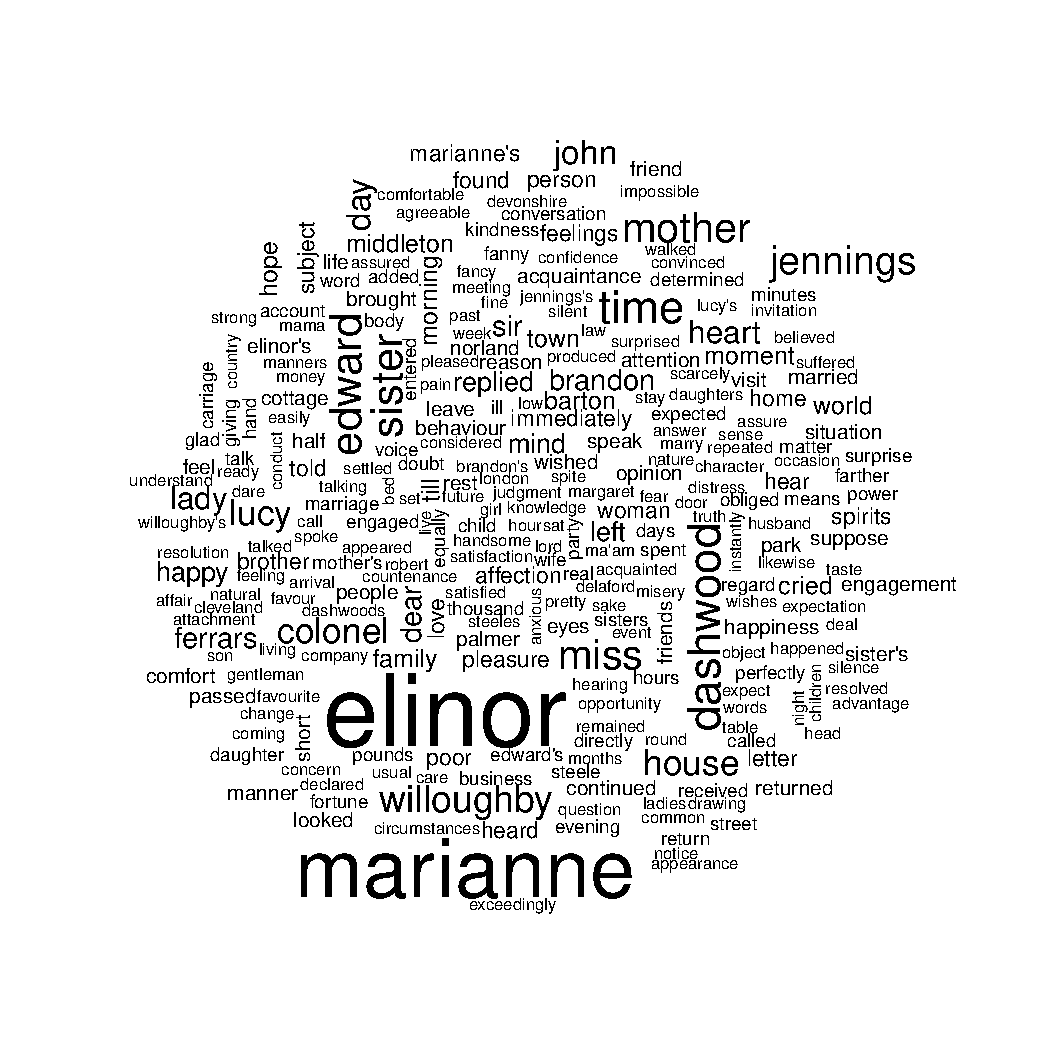
\includegraphics[width=\maxwidth]{figure/unnamed-chunk-8-1} 

\end{knitrout}


\bibliographystyle{apa}
\bibliography{article}
\nocite{*}
\end{document}
